\section{Présentation de la plateforme expérimentale}
\subsection{Pepper, un robot humanoïde à roues omnidirectionnelles}

\begin{figure}[!ht]	
	\begin{center}
		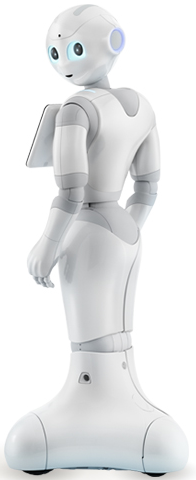
\includegraphics{juju}
		\caption{Pepper}
	\end{center} 
\end{figure}	

Présenter le robot, ces dimensions et caractéristiques physiques.\\
Parler de sb et de l'utilisation prévue des robots.

	
\subsection{Capteurs et actionneurs}

Présenter les différents capteurs et actionneurs, et leurs conséquences sur le contrôle du robot.

\subsection{Propriétés mécaniques}	

Parle de la base omnidirectionelle.\\
Présenter les roues.\\
Parler du jeu mécanique dans les articulations.\\
Présenter le problème de basculement.


\section{État de l'art}
\subsection{Problématiques associées à Pepper}

Présenter les différentes problématiques.\\
Montrer qu'elles sont similaires aux robots à roues et bipèdes.\\
Montrer les différences entre Pepper et ces robots.


\subsection{Commande et équilibre des robots à roues}
\subsubsection{Les robots à une et deux roues}

Présenter quelques articles.\\
Expliquer pourquoi les solutions proposées ne sont pas applicables, même pour le push recovery.

\subsubsection{Les robots à trois roues et plus}

Présenter quelques articles.\\
Montrer le fait que ces robots sont souvent considérés dynamiquement stable.\\
Pour ceux dont on considère le basculement, montrer que le système mécanique de ces robots implique que toute les roues sont en contact avec le sol.\\
Conclure en disant que le sujet de changement de nombre de roue a été peu traité.

\subsection{Commande et équilibre des robots bipèdes}

Présenter quelques articles (marche et push).\\
Montrer les similitudes (cop) et les différences (pied/base).

\subsection{Synthèse et conclusion}

Synthétiser les différentes sections.\\
Conclure de l'importance de la prédiction dans le contrôle de l'équilibre.\\
Nécessité de contrôler différents mode dynamiques (2 roues/3 roues au sol).\\
Besoin de contrôler à la fois le haut du corps et la base mobile.


\section{Organisation du document}

Document en deux parties : contrôle de l'équilibre sur 3 roues / Solution pour le problème du push recovery